\colorbox{white!10!}{
    \begin{minipage}{0.2\textwidth}
       \begin{flushleft}
        \includegraphics[width = 0.6\textwidth]{Эмблема.png}
       \end{flushleft}
    \end{minipage}
    \begin{minipage}[t]{0.7 \textwidth}
        \begin{center}
            {\huge \textsc{Красноярская Летняя Школа. Сезон $7^2 - 2$}}
            \vspace{0.25cm}
            
            { \huge \textbf{ФМТ. Финал}}
        \end{center}
        \vspace{0.05cm}
    \end{minipage}
}

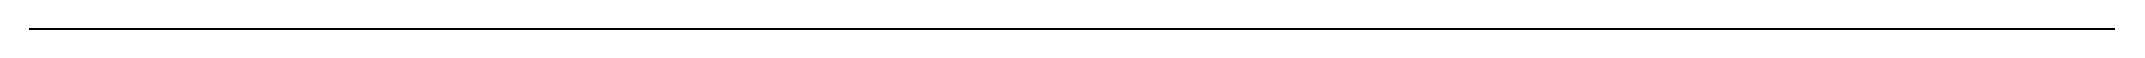
\begin{tikzpicture}
    \draw[thick] (-6.5,0)--(20,0);
\end{tikzpicture}
\begin{enumerate}
    
    
    \item Во вращающейся с постоянной скорость  $\omega$ карусели радиуса $r$ располагается мальчик, он бросает шарик с определённой скоростью $v$ таким образом, что тот ловит его, находясь в диаметрально противоположной точке. Определите допустимые значения скорости $v$. \\

    
   \parbox[b]{.7\textwidth}{%
    \item Cообразительный сотрудник с помощью небольшого грузика «подвесил» к наклонному потолку воздушный шарик (см. рисунок). Грузик какой массы $M$ годится для этой цели? При решении задачи считайте, что шарик имеет форму сферы радиусом $R$, проскальзывания нет, маcca peзиновой оболочки шарика $m$, плотность газа внутри шарика $\rho$, плотность атмосферы $\rho_0$, потолок имеет угол наклона $\alpha$.
    }\hfill\includegraphics[width=.3\textwidth]{pictures/Final_2.png}

\end{enumerate}